\chapter{Literature Review} \label{chapter:related-work}
% purpose of the review and search criteria
The literature review aimed at identifying work that was directly related to version control systems and their usability. The search for literature was based on three main criteria: (1) work that produced specific results that could also be utilized for this project, (2) work that was concerned with the interfaces of VCSs or the usability and (3) work that investigated the use of version control outside of the programming realm.

% review in context of the thesis
The reviewed literature was key to create a foundation for the research described in this thesis. The first design iteration has drawn heavily on the insights gained through the review, which is described in more detail in Section \ref{sec:git-feature-comparison}. Furthermore, this review provides the necessary context in which the results of this thesis should be seen and enables the reader to assess the contribution of this work to the current state of research.

\section{Usability of Version Control Software}
During the 2011 Git User Survey participants were asked which parts of Git needed improvement. A total of 73\% stated that  the user interface needs improvement \cite{_git_2011}. With this in mind, it is surprising how little research there is about the usability of version control systems in general and Git in particular. The two most notable studies have investigated the user experience as well as the conceptual design of different version control systems, among them Git \cite{church_case_2014,perez_de_rosso_whats_2013}.

Church, Söderberg and Elango have conducted an empirical study on the usage of command line-based version control inside two large IT companies (Google \& Autodesk) \cite{church_case_2014}. The study was based on interviews and observations within these companies. Engineers who participated covered a diverse range of job positions and had varying experience. The study results show that common usage patterns emerge when version control systems such as Git or Subversion are incorporated into the software development workflow. In both companies, most engineers stuck to a small set of commands and showed a general risk aversion when using version control. Church et al. note that the observed "ritualistic behaviour" of engineers is usually found among novice computer users and attribute this behaviour to a low user confidence in the version control systems used. They conclude that it is particularly problematic for a tool whose main premise it is to offer "development without fear" to be perceived as risky to use.

Explaining these results, Church et al. present a cognitive dimensions analysis of Git. They point out that there are many \textit{hidden dependencies}, such as between files and branches, local and remote repositories as well as between untracked files and the repository. Moreover, Git has an "abstraction barrier", meaning that certain concepts, i.e. branching, need to be learned, before the system can be used in a meaningful way. The authors reason that a combination of hidden dependencies and abstraction mostly contribute to the aforementioned usability problems. These conceptual issues are also the reason why the \ac{GUI} client by Github\footnote{https://mac.github.com/} only offers a slight improvement in usability. It makes features more discoverable and offers a more visually pleasing interface, but it suffers from the same deficiencies as the command line interface. The authors close by highlighting that the discovered issues need to be solved before version control can take the leap from computer science to a wider audience.

The second study mentioned above, by Jackson and Perez De Rosso \cite{perez_de_rosso_whats_2013}, was based on an analysis of Git's conceptual model. The researchers present the weaknesses in Git's conceptual design and propose an improved alternative called Gitless.

They argue that concepts have a strong influence of how users think about an application and therefore conceptual integrity should be an important consideration in software design. By concepts the researchers mean \emph{"the constructs and notions [...] that are invented for the purpose of structuring the functions of the system"} \cite[p.~38]{perez_de_rosso_whats_2013}. Git's concepts were scrutinized based on three main criteria that were defined by Frederick Brooks in the 1970s \cite{brooks_mythical_1995} and which he believed to be central to conceptual integrity. 1. orthogonality – individual concepts should be independent from each other, 2. propriety – a software should only have the essential functions that are needed for its operation, and 3. generality – a function should be applicable in different ways. After formally describing Git's main concepts the researchers go on in explaining which concepts violate these criteria and why. Regarding the first criterion, orthogonality, the researchers point out that Git's different file states, such as modified, staged and committed, are particularly troublesome. Commands that are primarily intended to modify one state, sometimes also affect the other. For example, if a user modifies a file, stages it and then goes on modifying the same file, the command git commit \textit{file} will commit both states of the file (the staged and the unstaged). This happens, even though the commit command typically only effects the staging area, unless told otherwise by a particular flag.
According to the researchers, the staging area also violates the second criterion – propriety. They argue that an intermediate step between editing and committing is rarely useful and that most users just want to commit their changes right away. Although this is possible through an additional flag (commit -a) this approach has some drawbacks as well, e.g. that untracked files will not be included in the commit and that a high verbosity is required when committing only a few files.
The last criterion, generality, is violated by the branch concept. Even though branches allow users to save different parallel versions of a file, this concept does not apply to the working directory or the staging area. There is only one working directory and one staging area. This means that changes made to a file need to be committed before branches can be switched. This is unnecessarily troublesome and requires the use of another function (git stash) in case the user does not want to commit a file, because the code is in a broken state for example.

Concluding, Jackson and Perez de Rosso suggest that software is designed from inside out and that interfaces can only be as good as the underlying concepts. Therefore, they propose a simplified \ac{CLI} for Git, called Gitless \footnote{http://gitless.com}, that eliminates the aforementioned issues. Among other things the staging area was removed and a more general branch concept got introduced. Gitless is an open-source project that is built on top of Git. The researchers hope that it will be further improved by the community and that it sparks a discussion on how version control can be made simpler and more user-friendly.

The results of this study can partially explain why the engineers interviewed for the study by Church et al. \cite{church_case_2014}
acted so risk-averse when using Git. The inconsistencies throughout the system might have prevented them from forming an accurate mental model.

\section{Proposed Improvements to Version Control}
Gitless is not the only attempt to make version control systems easier to use. The official Git Wiki lists as many as 36 different GUI clients for Git\footnote{https://git.wiki.kernel.org/index.php/InterfacesFrontendsAndTools}, whose main goal it is to make version control simpler and more accessible. Jackson and Perez De Rosso claim that these interfaces merely add an aesthetic layer to Git, but fail to make it simpler, because they are still operating within the boundaries of Git's inherent concepts. Below, projects are described that tried to dismiss these boundaries by looking into new ways of approaching version control.

Bicer, Koc and Tansel note that even though version control was supposed to make collaboration  easier, it only does so as long as there are no conflicting changes \cite{koc_towards_2012}. But so called merge conflicts happen regularly during the development process. They can only be resolved by direct communication between the engineers who are responsible for the changes. This works well as long as both engineers share the same location, but nowadays large companies span the whole globe and open source projects are being developed by a diverse group of people from all around the world. Bicer et al. state that most version control systems do not offer a platform for resolving these merge conflicts. They suggest the introduction of a new command, called \textit{peek}, which allows developers to take a look at local changes of other contributors in order to prevent conflicts from happening in the first place. The feature is accompanied by a social networking site that is believed to encourage communication between developers.

Even though Bicer et al. identified what seems to be a common problem with version control systems \cite{apel_semistructured_2011,brosch_guiding_2010,guimaraes_improving_2012}, their solutions did not succeed in reducing the number of conflicts. During a small experiment with 5 developers the users of the system were reluctant to utilize the new peek feature. The researchers blame the laborious process of having to request a peek first and the necessity of monitoring changes of colleagues regularly.

\setlength{\parskip}{1em}
\noindent Because of the usability shortcomings of version control a solution to automate it entirely has been proposed \cite{weber_automatic_2012}. The thesis describes a web-based IDE (Integrated Development Environment) that avoids conflicts by implementing an elaborate change awareness system. This system will warn developers in case they try to change code that team members are working on as well. The IDE utilizes different colors to highlight sections that are conflicting. When a conflicting line is highlighted, the user has the option to adopt the changes of a collaborator first and base her subsequent work on this updated state. This means that conflicts can be avoided right from the start and reduces the need for laborious conflict resolution during the merge process.

\setlength{\parskip}{0em}
This mechanism is enabled by a feature called \textit{AutoShare}, which basically means that changes are saved, committed and pushed automatically without any user interaction. Through this, users get a real-time view of what their collaborators are working on. This enables remote pair-programming for example, among other things. For programmers who prefer a more granular control all version control features can also be operated manually.

Even though case studies have been described, no user tests were performed as part of the thesis. This makes it hard to gauge whether the proposed solution could be potentially adopted by programmers. Eventual downsides of the proposed solution are a harder to navigate project history, because automated commit messages might not be as descriptive, and a possibly too disruptive IDE. For example if a developer consciously decides to ignore conflicting changes and the system keeps warning her.% this is my own conclusion

\section{Version Control Outside of Software Development}
Given its usefulness it is surprising that version control has not become ubiquitous yet. As Grischenko notes, versioning was even part of the original hypertext concept \cite{grishchenko_deep_2010}, but today it is mostly found in highly specialized areas where collaboration on large sets of text-based documents takes place. Besides software development this is particularly digital publishing, where the emergence of Wikis has exposed the concept to a larger audience \cite{priedhorsky_wiki_2011}. Within this area it is usually referred to as revision control (Wikipedia, to stay inside the subject matter, treats the terms revision control, version control and source control as synonymous\footnote{https://en.wikipedia.org/wiki/Revision\_control}). The utilization of version control inside wikis is not surprising, since the process of creating a wiki holds similar requirements as the software development workflow. (1) collaboration is very common, therefore (2) concurrent editing is an essential feature and (3) transparent edits should allow reviewing and reverting changes if necessary \cite{priedhorsky_wiki_2011}. % the history for wikis is the "recent changes" page, maybe mention that?

Version control is especially hard to find in consumer products. The most prominent examples might be the \textit{track changes} feature of Microsoft Word \cite{thede_track_2009} and Google Docs revision history\footnote{https://support.google.com/docs/answer/190843}. Both are automated version control systems that allow users to go back in time and look at different revisions of a document or changes that were introduced by collaborators.

When looking beyond publishing and text processing version control systems are less common. This might be due to the increased complexity of implementing version control for other domains. Computing and visualizing differences between text-files is much easier than for example between binary files on which most graphical and video file formats depend.  There have been several attempts of bringing version control to graphics\footnote{https://blogs.adobe.com/jnack/2009/03/new\_version\_control\_system\_for\_photoshop.html} \footnote{http://adobe.wikia.com/wiki/Adobe\_Version\_Cue} \footnote{http://www.alienbrain.com/}. Most of them have used a rather simplistic approach, storing revisions as individual files. Thus, the user gets a temporal history of changes, but is not able to look at a delta of two revisions, because the system is blind to the semantics of changes.

A more advanced version control system for graphics has been proposed by Chen, Wei and Chang \cite{chen_nonlinear_2011}. The researchers implemented a non-linear revision control system for GIMP, an open source graphical editing tool\footnote{http://www.gimp.org/}. In order to offer a meaningful revision history the system records high-level user interactions. Based on these a graph-based representation is created that allows users to review spatial, temporal and semantic relations between different revisions. Nodes represent image editing operations whereas edges represent the relationship between these. On top of that, the graph nodes provide small thumbnails so that users can spot differences between revisions at a glance (Figure \ref{fig:gimp-rev-control}).

\begin{figure}[h!]
 \centering
 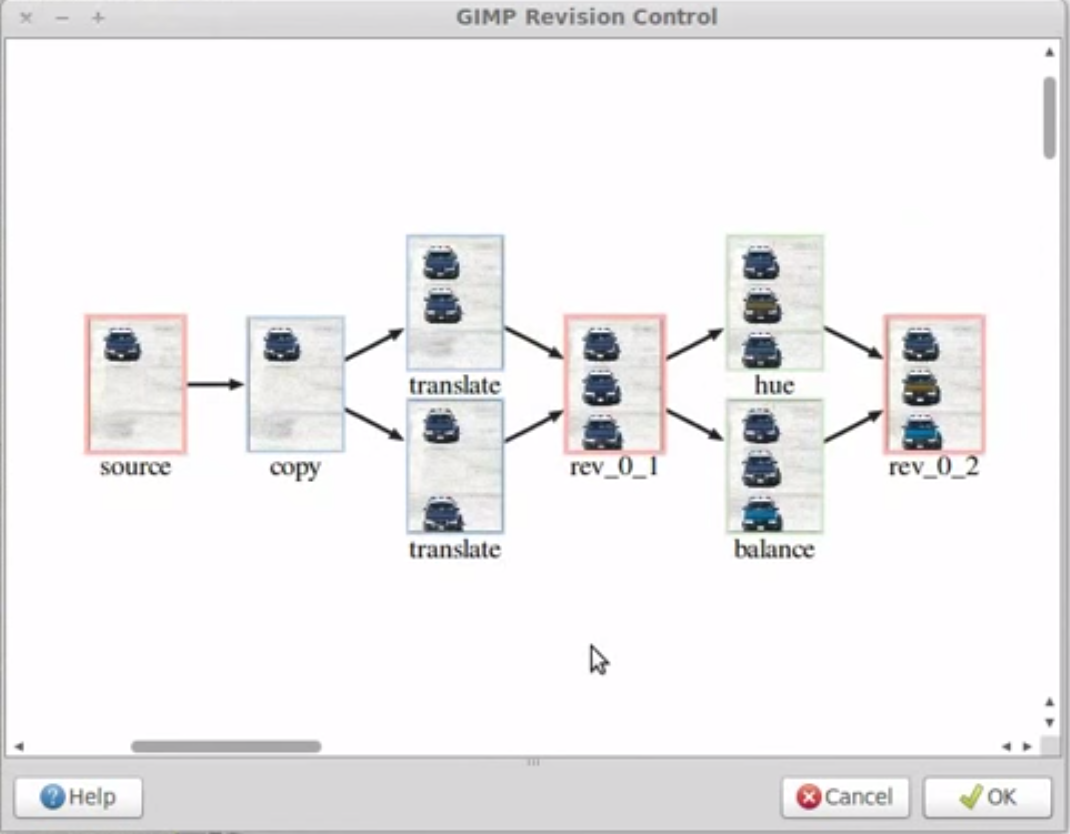
\includegraphics[width=12cm]{related-work/gimp-revision-control}
 \caption{Revision control for GIMP, screenshot taken from introductory video \cite{_nonlinear_????}.}
 \label{fig:gimp-rev-control}
\end{figure}

% source of image:
% how to reference?
% http://www.ht-timchen.com/research/nonlinear-revision-control-for-images/

The system enables users to navigate different versions of a graphics file, compare them (diff) as well as create new branches and merge changes. Furthermore, the user can manually check in new revisions, even though this is generally unnecessary since the system tracks all user actions automatically. Common use cases cited by the researchers are image editing and digital sketching. Especially the latter one often involves trial-and-error experiments that make revision control particularly useful. During usability tests Chen et al. found that participants were happy to integrate revision control features into their workflow. Especially the visual representation of the history was deemed useful. Merging on the other hand, seemed to be more difficult for some users. The researchers conclude that even though the system is easy to use and helpful it might take some time and practice to master it.

\section{Conclusion}
It seems like most research in the area of version control is concerned with the shortcomings of different systems, both in terms of usability and the conceptual design. In some research projects alternative solutions have been investigated, but those are usually situated within the programming realm. Unfortunately, there are not many examples in which version control has been applied to other domains. In general, most research is focused on the widely used open source VCSs Git and Subversion.

It has become apparent that Git has some conceptual deficiencies that cannot be solved by just creating a new interface. Instead the underlying structure needs to be questioned and features should be redesigned or dismissed. The fact that experienced engineers at renowned software companies were anxious to freely interact with the system is proof that Git has some design flaws. These problems need to be eliminated before Git can be used by a non-technical audience.

On the other hand, fully automated version control does not seem to be the holy grail either. If users are not exposed to version control features at all it decreases the discoverability and might prevent them from forming an accurate mental model of the system. This might handicap their ability to solve problems in case the system does not work as intended. Furthermore, automated version control lacks a fine-grained control of how the work is structured and presented to collaborators (commit messages and history).

The findings of Bicer et al. showed that not every problem a software has can be fixed by adding new features. Sometimes, designers and researchers are better off accepting the boundaries of what software can achieve and focusing on building a lean system that can do everything that is necessary but not more than that. This again highlights the importance of \textit{propriety}, offering only the smallest possible set of features, mentioned by Jackson and Perez De Rosso. Nevertheless, facilitating communication through a version control system is a promising and important feature that should not be ruled out, only because it did not work in one particular setting.

Concluding one could say that Git's conceptual design flaws need to be eliminated and that hidden dependencies should be reduced. Section \ref{sec:git-feature-comparison} describes in more detail how this review influenced the design of the first prototype. Chapter \ref{chapter:focus-group} outlines how some of the inconsistencies were addressed.

% This will be a challenging task given that the new system will still be based on Git and Github. Nevertheless, Jackson and Perez de Rosso have shown that enhancements can be made even within the constraints of an existing system.

% State of the Art is described in correct technical and business­-related terms?
% ­Search strategy for literature is explicit and rational?
% ­Quality of the literature analysis: broad and profound (e.g. more articles used)?
% ­Recent and important literature concerning state­ of ­the ­art?
% ­Report gives sufficient arguments to what degree literature can inform the current practice?
% ­Report gives sufficient arguments why findings from current literature can/cannot be applied to innovation project?
% ­Report describes about what clarifications and modifications on concepts from literature need to be taken into account so that findings from current literature become applicable?
